\documentclass[tikz,border=10pt]{standalone}
\usepackage[T1]{fontenc}
\usepackage{mathpazo}
\usepackage{amsmath,amssymb}
\usetikzlibrary{arrows.meta, positioning, calc, decorations.markings}

\definecolor{stblue}{HTML}{7B97AD}
\definecolor{rwgold}{HTML}{B8995E}
\definecolor{sage}{HTML}{7A9A7E}
\definecolor{dkbrown}{HTML}{3D3530}
\definecolor{wmgray}{HTML}{7B7067}
\definecolor{cream}{HTML}{F9F6F0}
\definecolor{border}{HTML}{D4C9B8}

\begin{document}
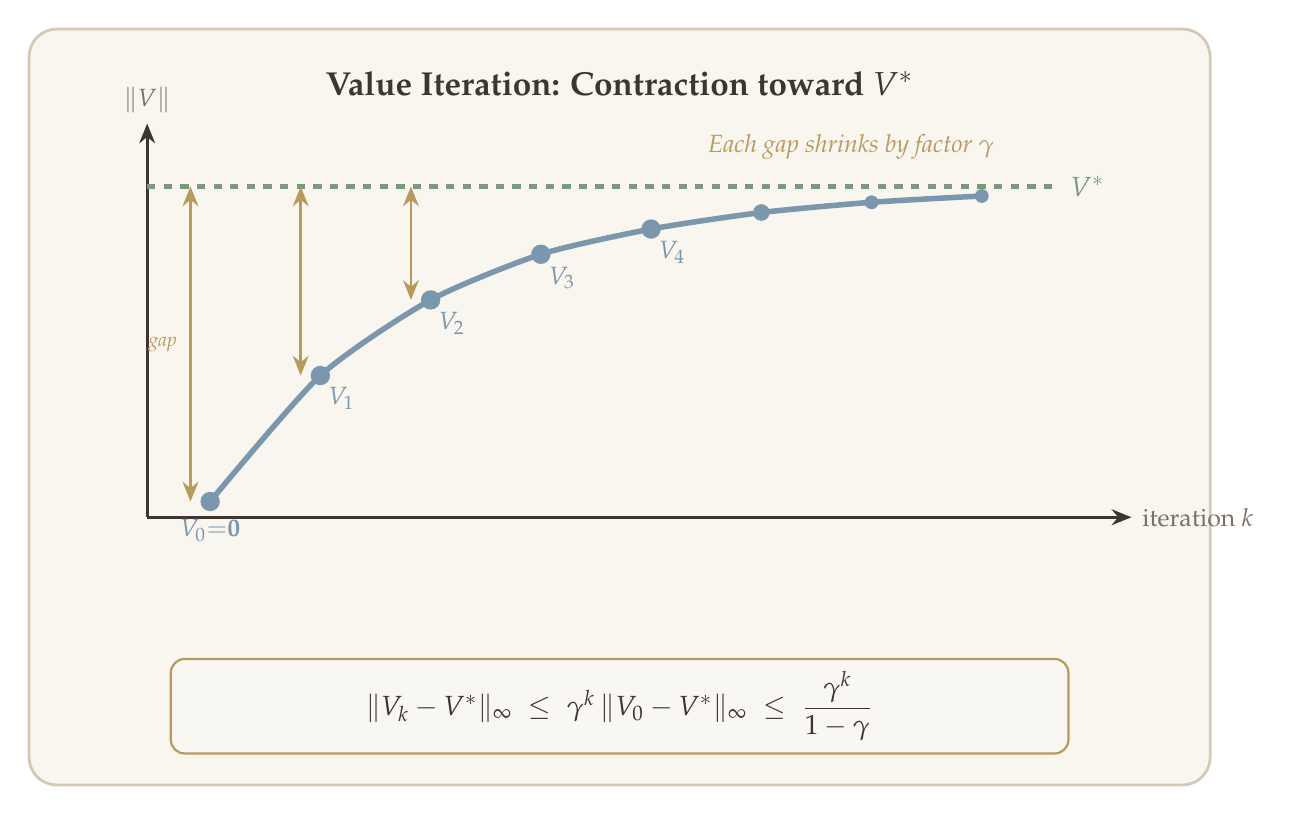
\begin{tikzpicture}[
  >={Stealth[length=2.5mm, width=2mm]},
]

% Background
\fill[cream, rounded corners=10pt] (-1.5,-3.6) rectangle (13.5,6.0);
\draw[border, rounded corners=10pt, line width=1pt] (-1.5,-3.6) rectangle (13.5,6.0);

% Title
\node[font=\large\bfseries, text=dkbrown] at (6.0,5.3)
  {Value Iteration: Contraction toward $V^*$};

% === Axes ===
\draw[->, line width=1.2pt, dkbrown] (0,-0.2) -- (12.5,-0.2)
  node[right, font=\small, text=wmgray] {iteration $k$};
\draw[->, line width=1.2pt, dkbrown] (0,-0.2) -- (0,4.8)
  node[above, font=\small, text=wmgray] {$\|V\|$};

% === V* horizontal dashed line ===
\draw[sage, line width=1.8pt, dashed] (0,4.0) -- (11.5,4.0);
\node[font=\normalsize\bfseries, text=sage, anchor=west] at (11.6,4.0) {$V^*$};

% === Data points (V_k converging to V*) ===
% V* is at y=4.0, V_0=0 at y=0.0
% V_k = V* (1 - gamma^k), with gamma=0.6 for visual appeal
% y_k = 4.0 * (1 - 0.6^k)
% k=0: 0.00, k=1: 1.60, k=2: 2.56, k=3: 3.14, k=4: 3.46
% k=5: 3.67, k=6: 3.80, k=7: 3.88, k=8: 3.93

\coordinate (V0) at (0.8, 0.0);
\coordinate (V1) at (2.2, 1.60);
\coordinate (V2) at (3.6, 2.56);
\coordinate (V3) at (5.0, 3.14);
\coordinate (V4) at (6.4, 3.46);
\coordinate (V5) at (7.8, 3.67);
\coordinate (V6) at (9.2, 3.80);
\coordinate (V7) at (10.6, 3.88);

% Curve through points
\draw[stblue, line width=2pt, smooth, tension=0.4]
  plot coordinates {
    (0.8, 0.0)
    (2.2, 1.60)
    (3.6, 2.56)
    (5.0, 3.14)
    (6.4, 3.46)
    (7.8, 3.67)
    (9.2, 3.80)
    (10.6, 3.88)
  };

% Points
\fill[stblue] (V0) circle (3.5pt);
\fill[stblue] (V1) circle (3.5pt);
\fill[stblue] (V2) circle (3.5pt);
\fill[stblue] (V3) circle (3.5pt);
\fill[stblue] (V4) circle (3.5pt);
\fill[stblue] (V5) circle (3pt);
\fill[stblue] (V6) circle (2.5pt);
\fill[stblue] (V7) circle (2.5pt);

% Labels
\node[font=\small\bfseries, text=stblue, below] at (0.8,-0.1) {$V_0{=}\mathbf{0}$};
\node[font=\small, text=stblue, below right=-1pt] at (2.2,1.55) {$V_1$};
\node[font=\small, text=stblue, below right=-1pt] at (3.6,2.50) {$V_2$};
\node[font=\small, text=stblue, below right=-1pt] at (5.0,3.08) {$V_3$};
\node[font=\small, text=stblue, below right=-1pt] at (6.4,3.40) {$V_4$};

% === Contraction gap arrows ===
% Gap from V0 to V*
\draw[rwgold, line width=1pt, <->] (0.55, 0.0) -- (0.55, 4.0);
\node[font=\scriptsize\itshape, text=rwgold, anchor=east] at (0.5, 2.0) {gap};

% Gap from V1 to V*
\draw[rwgold, line width=0.9pt, <->] (1.95, 1.60) -- (1.95, 4.0);

% Gap from V2 to V*
\draw[rwgold, line width=0.8pt, <->] (3.35, 2.56) -- (3.35, 4.0);

% === Shrinkage annotation ===
\node[font=\small\itshape, text=rwgold, anchor=west] at (7.0,4.5)
  {Each gap shrinks by factor $\gamma$};

% === Bottom formula box ===
\draw[rwgold, line width=0.8pt, rounded corners=5pt, fill=rwgold!8]
  (0.3,-3.2) rectangle (11.7,-2.0);
\node[font=\normalsize, text=dkbrown] at (6.0,-2.6)
  {$\|V_k - V^*\|_\infty \;\leq\; \gamma^k \,\|V_0 - V^*\|_\infty \;\leq\; \dfrac{\gamma^k}{1 - \gamma}$};

\end{tikzpicture}
\end{document}
